\renewcommand{\theequation}{\theenumi}
\begin{enumerate}[label=\thesection.\arabic*.,ref=\thesection.\theenumi]
\numberwithin{equation}{enumi}

\item 
\begin{align}
\vec{A}=\myvec{-3\\10}
\vec{B}=\myvec{6\\-8}
\vec{C}=\myvec{-1\\6}
\end{align}
Let $\vec{C}$ divide AB in ratio k:1.Then by section formulae,
\begin{align}
\vec{C}=\frac{k\vec{B}+\vec{A}}{k+1}
\\
\myvec{-1\\6}=\frac{1}{k+1}\myvec{6k-3\\-8k+10}
\\
k=\frac{2}{7}
\end{align}
So $\vec{C}$ divides AB in ratio 2:7
\newline
The following Python code generates Fig. \ref{fig:section}
%
\begin{lstlisting}
codes/line/section/section.py
\end{lstlisting}
\begin{figure}[!ht]
\centering
\includegraphics[width=\columnwidth]{./codes/line/section/pyfigs/section.eps}
\caption{C divides AB in ratio k:1}
\label{fig:section}
\end{figure}
\end{enumerate}
